\section{Gist}

There are much more concepts than shown below in the original gist upper ontology, however, the figure 
is to illustrate some of the useful concepts that have been used in the project. More specifically, 
concepts of \textbf{ID}, \textbf{Text}, \textbf{Language} and relations of \textit{is expressed in}, 
\textit{is part of}, \textit{unique text}, \textit{contained text} have been integrated into the project.

\begin{figure}[ht]
	\centering
	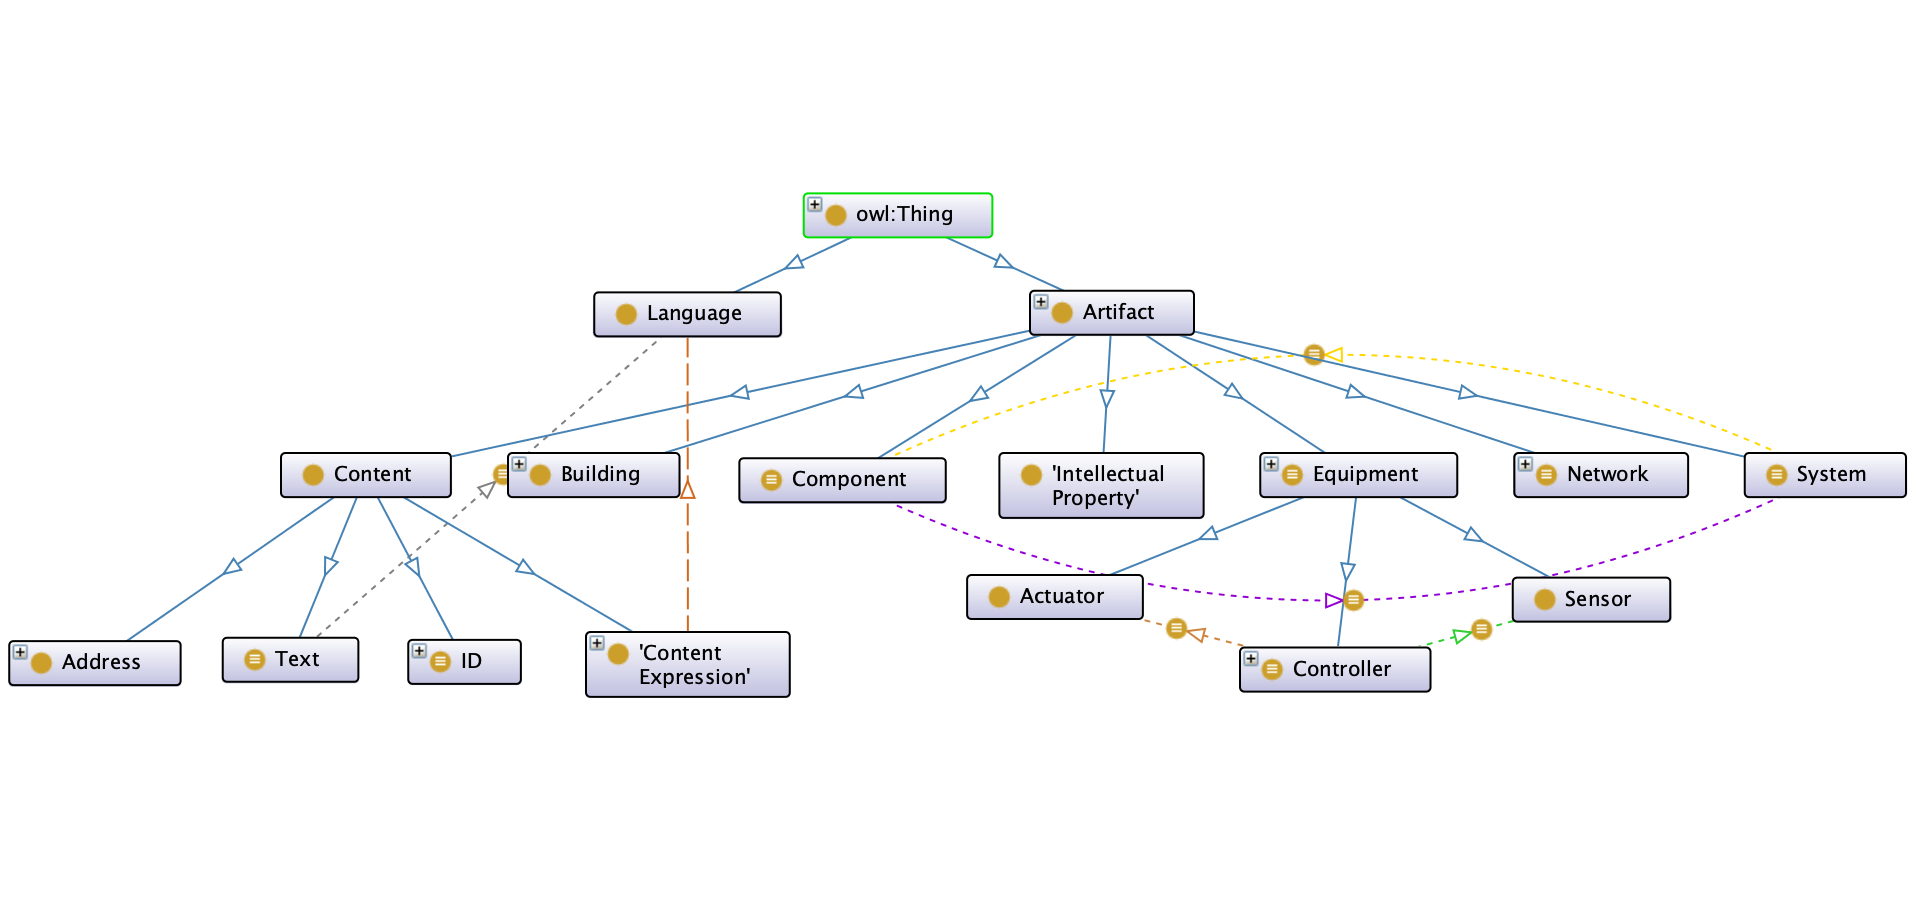
\includegraphics[width=\textwidth]{../../resources/gist_view.png}
	\caption{gist view}
	\label{fig:gist_view}
\end{figure}

\section{OTTR}

\begin{figure}[H]
	\centering
	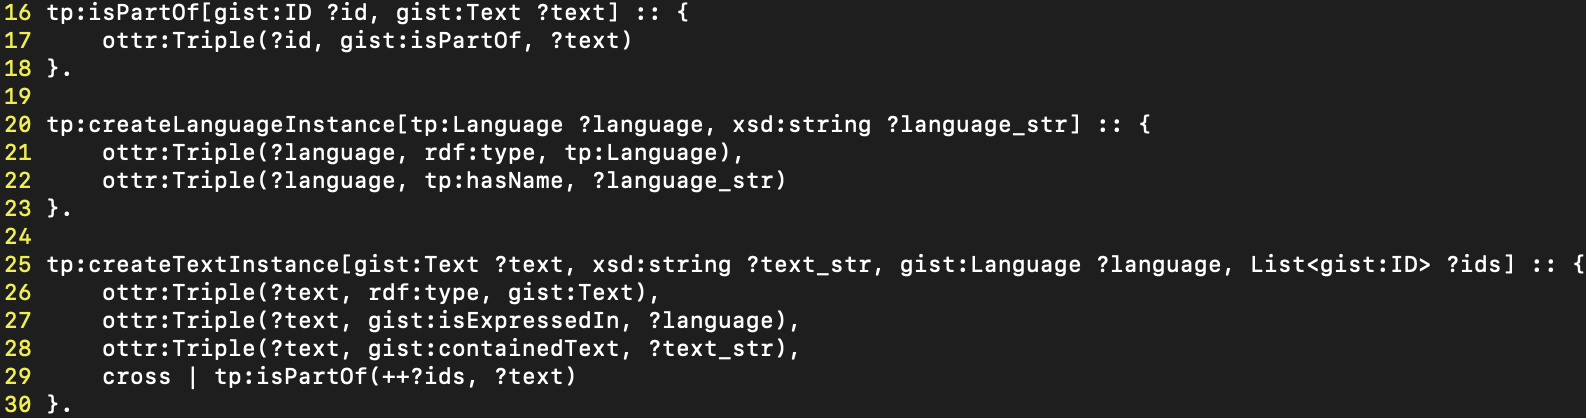
\includegraphics[width=0.75\textwidth]{../../resources/ottr_lib_example.png}
	\caption{OTTR library example}
	\label{fig:ottr_library_example}
\end{figure}

\section{ETL}

\begin{figure}[H]
\begin{subfigure}{\textwidth}
  \centering

  \begin{table}[H]
	  \begin{tabular}{|p{0.40\linewidth}|p{0.25\linewidth}|p{0.31\linewidth}|}
		  \hline
		  \textbf{Subject} & \textbf{Predicate} & \textbf{Object} \\
		  \hline
		  \multirow{4}{*}{tp:PNLC1BL34U31} & rdf:type & tp:PartNumber \\
		   & gist:isIdentifiedBy & tp:IDLC1BL34U31 \\
		   & gist:isDescribedIn & tp:Text-6378022537900392513 \\
		   & tp:hasPartFamily & tp:PF90-22112018-056525 \\
		  \hline
		  \multirow{3}{*}{tp:PF90-22112018-056525} & rdf:type & tp:PartFamily \\
		   & gist:isIdentifiedBy & tp:ID90-22112018-056525 \\
		   & gist:isDescribedIn & tp:Text-2992260873777870348 \\
		  \hline
		  \multirow{3}{*}{tp:Text-6378022537900392513} & rdf:type & gist:Text \\
		   & gist:containedText & "TeSys B contactor 4P 800A 240V AC - LC1BL34U31" \\
		   & gist:isExpressedIn & tp:Language-def \\
		  \hline
	  \end{tabular}
	\end{table}
\end{subfigure}
\end{figure}

\begin{figure}[H]
\ContinuedFloat
\begin{subfigure}{\textwidth}
\centering

  \begin{table}[H]
	  \begin{tabular}{|p{0.40\linewidth}|p{0.25\linewidth}|p{0.31\linewidth}|}
		  \hline
		  \multirow{3}{*}{tp:Text-2992260873777870348} & rdf:type & gist:Text \\
		   & gist:containedText & "TeSys B contactor 4P 800A 240V AC" \\
		   & gist:isExpressedIn & tp:Language-def \\
		  \hline
		  \multirow{3}{*}{tp:IDLC1BL34U31} & rdf:type & gist:ID \\
		   & gist:uniqueText & "LC1BL34U31" \\
		   & gist:isPartOf & tp:Text-6378022537900392513 \\
		  \hline
		  \multirow{3}{*}{tp:ID90-22112018-056525} & rdf:type & gist:ID \\
		   & gist:uniqueText & "90-22112018-056525" \\
		   & gist:isPartOf & tp:Text-2992260873777870348 \\
		  \hline
		  \multirow{3}{*}{tp:ID4P} & rdf:type & gist:ID \\
		   & gist:uniqueText & "4P" \\
		   & gist:isPartOf & tp:Text-6378022537900392513 \\
		   & gist:isPartOf & tp:Text-2992260873777870348 \\
		  \hline
		  \multirow{3}{*}{tp:ID800A} & rdf:type & gist:ID \\
		   & gist:uniqueText & "800A" \\
		   & gist:isPartOf & tp:Text-6378022537900392513 \\
		   & gist:isPartOf & tp:Text-2992260873777870348 \\
		  \hline
		  \multirow{3}{*}{tp:ID240V} & rdf:type & gist:ID \\
		   & gist:uniqueText & "240V" \\
		   & gist:isPartOf & tp:Text-6378022537900392513 \\
		   & gist:isPartOf & tp:Text-2992260873777870348 \\
		  \hline
	  \end{tabular}
  \end{table}

\end{subfigure}
\caption{RDF/Turtle triples for ETL-1}
\label{fig:rdf_ttl_example_full}
\end{figure}

\section{Responding Knowledge Acquisition Software}

\subsection{Library usage}
\label{prog:library}
\begin{lstlisting}
from etl import *


class MyExtractor(Extractor):
	# your implementation

class MyTransformer(Transformer):
	# your implementation

class MyLoader(Loader):
	# your implementation


if __name__ == "__main__":
	# declaring an Extractor object
	extractor = MyExtractor(None)

	# declaring a Transformer object
	transformer = MyTransformer(None)

	# declaring a Loader object
	loader = MyLoader(None)

	# initializing OperationalData object
	data = OperationalData({})

	# initalizing ETL object
	etl = ETL(pipeline=[extractor, transformer, loader])

	# executing the ETL pipeline processes
	etl.run(data)
\end{lstlisting}

